The first model we present considers an elliptic cell with orientation $\theta$ placed within a
channel of infinite width and fixed height $H$. The setup for this model is illustrated
in Figure \ref{fig:model1_setup}.

\begin{figure}[htbp]
    \centering
    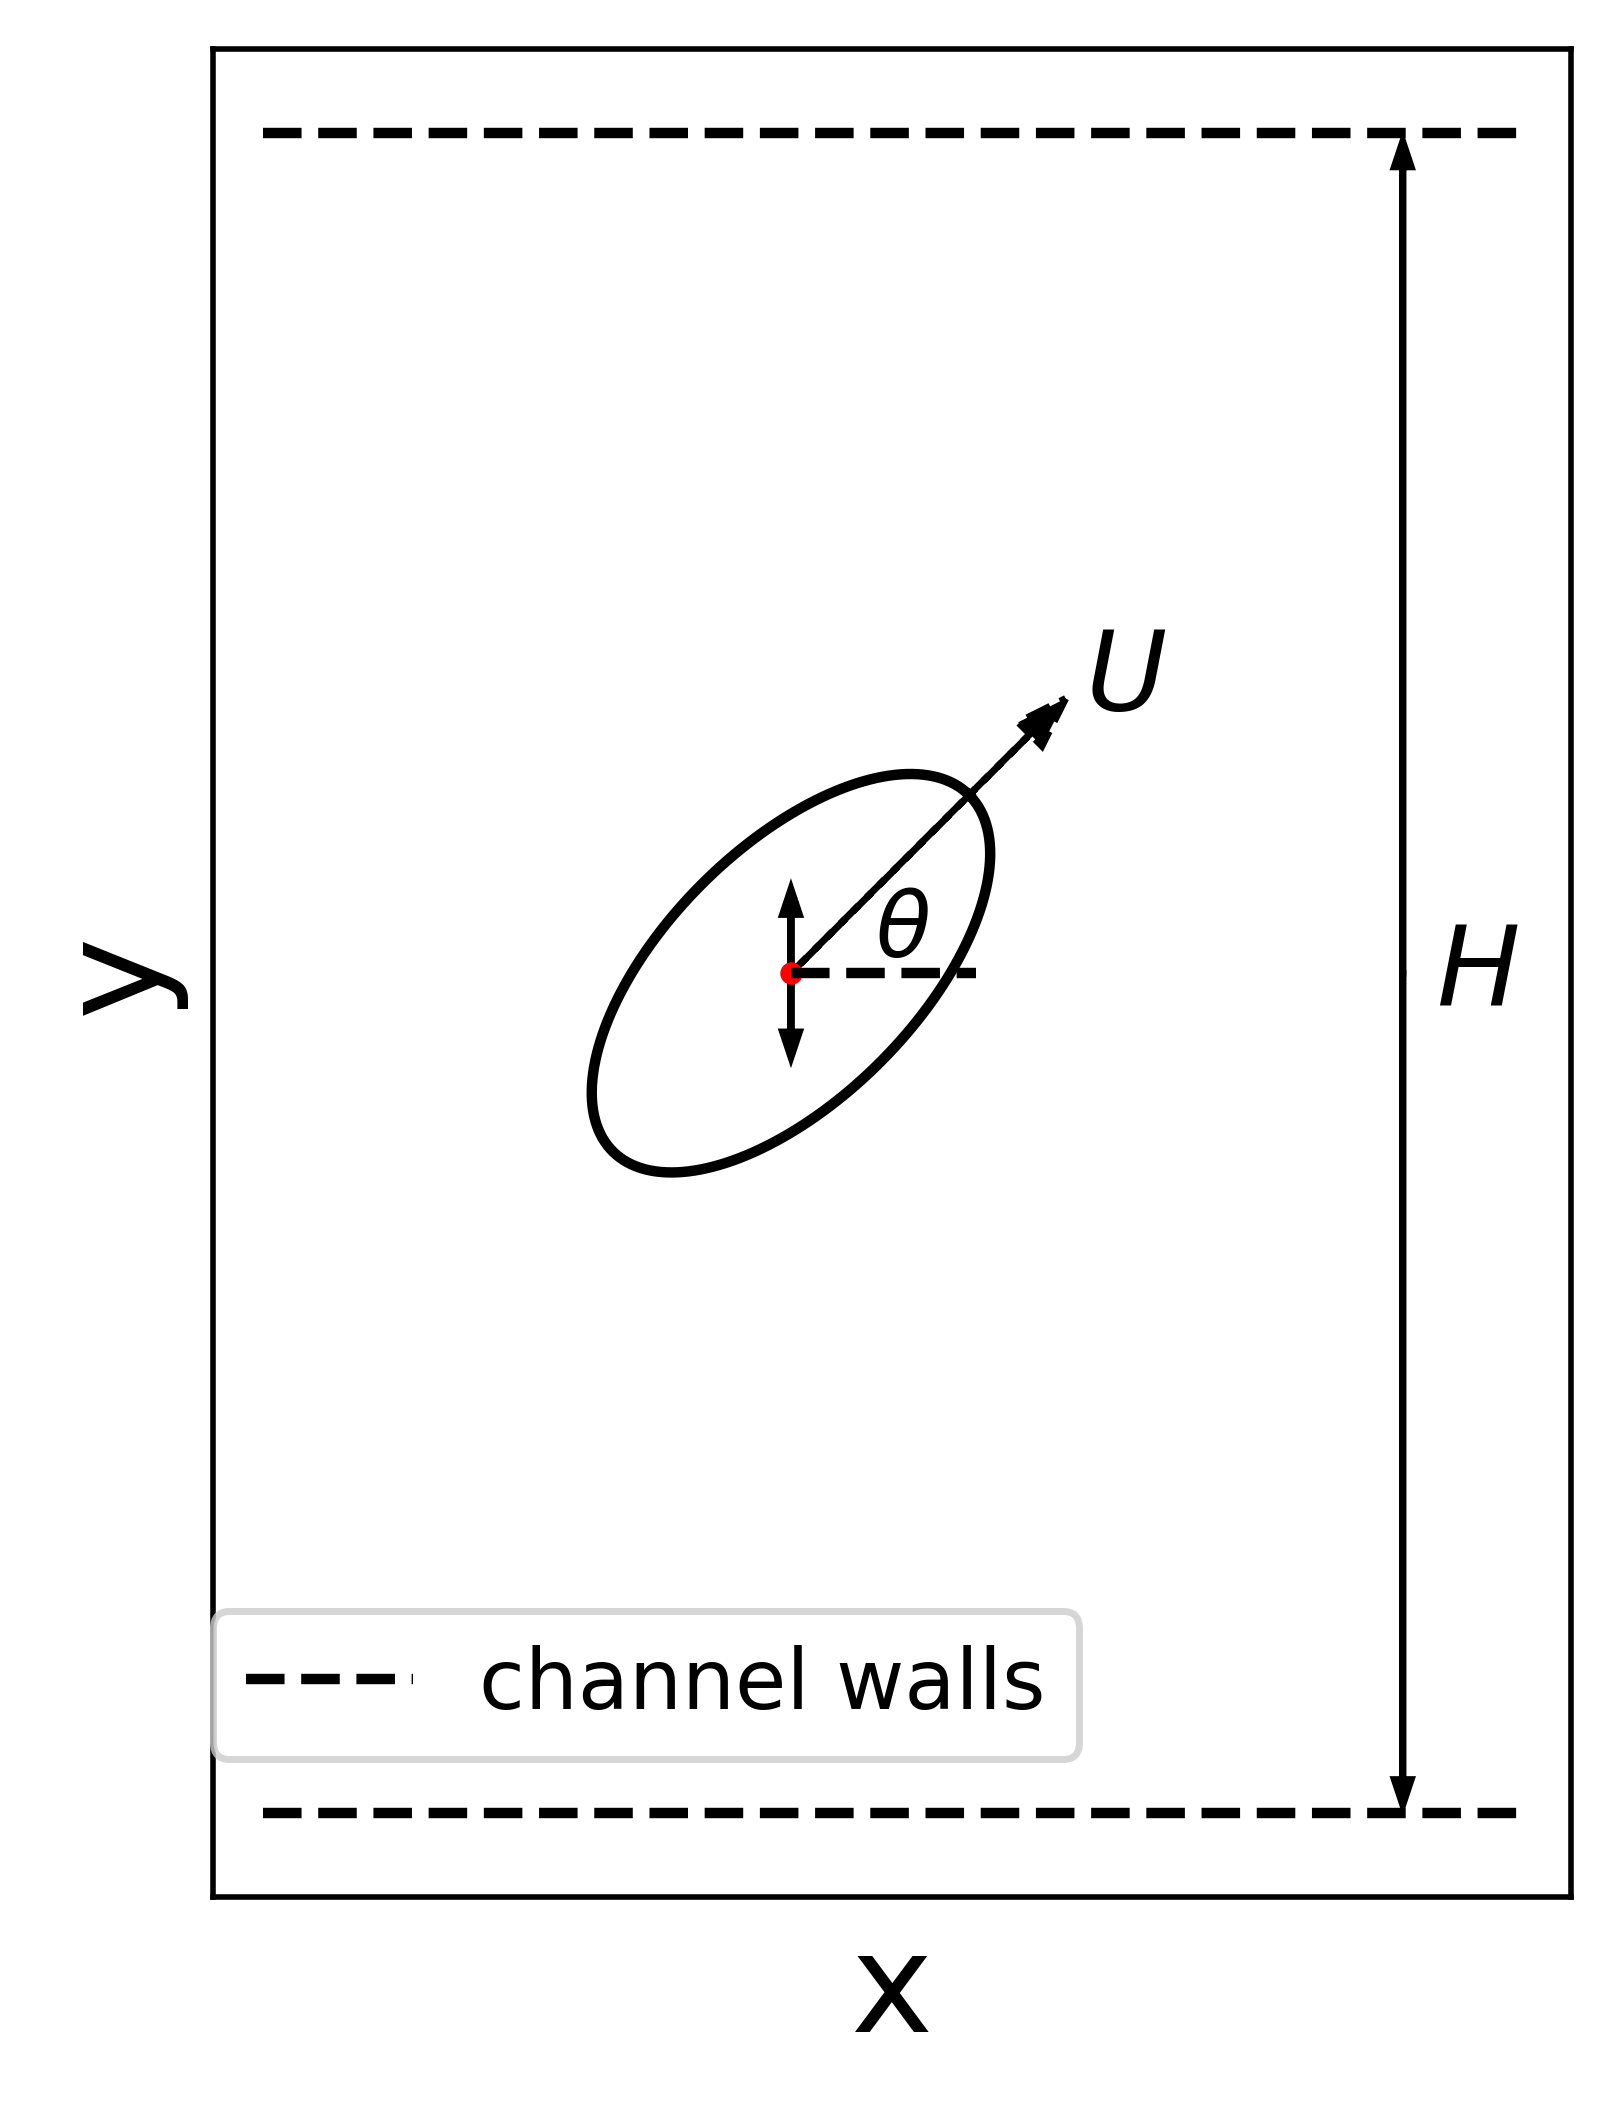
\includegraphics[scale=0.5]{graphics/model1_setup.png}
    \caption{An elliptic cell with orientation $\theta$ located within a channel of fixed height H
    and infinite width. The channel walls are considered reflective boundaries.}
    \label{fig:model1_setup}
\end{figure}

The dynamics imposed on the cell are described by the following coupled SDEs:

\begin{subequations}\label{eq:model1_sdes}
    \begin{align}
        Y(t + \Delta t) &= Y(t) + U \sin(\theta) + \sqrt{2D_y}\Delta W_1 \label{eq:model1_sdes_a} \\
        \theta(t + \Delta t) &= \theta(t) + \sqrt{2D_\theta}\Delta W_2 \label{eq:model1_sdes_b}
    \end{align}
\end{subequations}

Here, $Y(t)$ denotes the vertical position of the cell's geometric centre at time $t$,
and $\theta$ its orientation at that time. The parameters 
$D_y$ and $D_\theta$ scale the respective Brownian motion terms, modelling random
fluctuations in position and orientation. The parameter $U$ sets the deterministic speed 
of the cell's motion along the $y$-axis, thereby controlling the magnitude of the directed 
movement within the channel. We treat the upper and lower channel walls as 
reflective boundaries. Movement along the $x$-axis is disregarded, as our primary interest is in understanding
whether this system exhibits boundary accummulation behaviour. Given the channel's infinite extent along
the $x$-axis, horizontal movements have no meaningful impact on the boundary accumulation analysis. 
care primarily about whether this system exhibits boundary accummulating behaviour. With no bounds along $x$, 
it is irrelevant to consider movement along the $x$-axis. 

Our primary objective is to identify whether this system exhibits boundary accummulation behaviour. To
investigate this, we seek the stationary distribution - the long-term PDF to which the system converges as
$t \to \infty$. To obtain this stationary distribution, two approaches are available: Performing Monte Carlo 
simulations using equations \eqref{eq:model1_sdes}, or directly solving the corresponding Fokker-Planck PDE.

Both of these approaches however first require us to identify the configuration space of the system - the space of 
possible configurations of $y$ and $\theta$ the system can inhabit. As the cell's orientation $\theta$ is periodic
and thus unbounded, the vertical position $y$ is constrained by the channel walls. SPecifically, the minimum 
distance the centre of the clel can approach each channel wall depends expicitly on its orientation $\theta$. 
This dependency is illustrated in Figure \ref{fig:rolling_oval}.

\begin{figure}[htbp]
    \centering
    \includegraphics[scale=0.45]{graphics/rolling_oval.png}
    \caption{Path traced by the oval's centre, illustrating the minimum distance achievable to a horizontal
    wall as a function of orientation $\theta$}
    \label{fig:rolling_oval}
\end{figure}

The function characterising this minimum distance is termed the \textit{wall distance} function
\cite{chen2021shape}. For the specific case of an ellipse, this function is defined by:

\begin{subequations}\label{eq:wall_dist_funcs}
    \begin{align}
        y_{min}(\theta) &= \sqrt{a^2\sin^2(\theta) + b^2\cos^2(\theta)} \\
        y_{max}(\theta) &= H - \sqrt{a^2\sin^2(\theta) + b^2\cos^2(\theta)}
    \end{align}
\end{subequations}

where $a$ and $b$ are the major and minor semi-axes for the elliptic cell, respectively. 
Equations \eqref{eq:wall_dist_funcs} establish the upper and lower boundaries of the configuration space for this
system.Figure \ref{fig:configuration_space_model_1} illustrates the derived configuration space.

\begin{figure}[htbp]
    \centering
    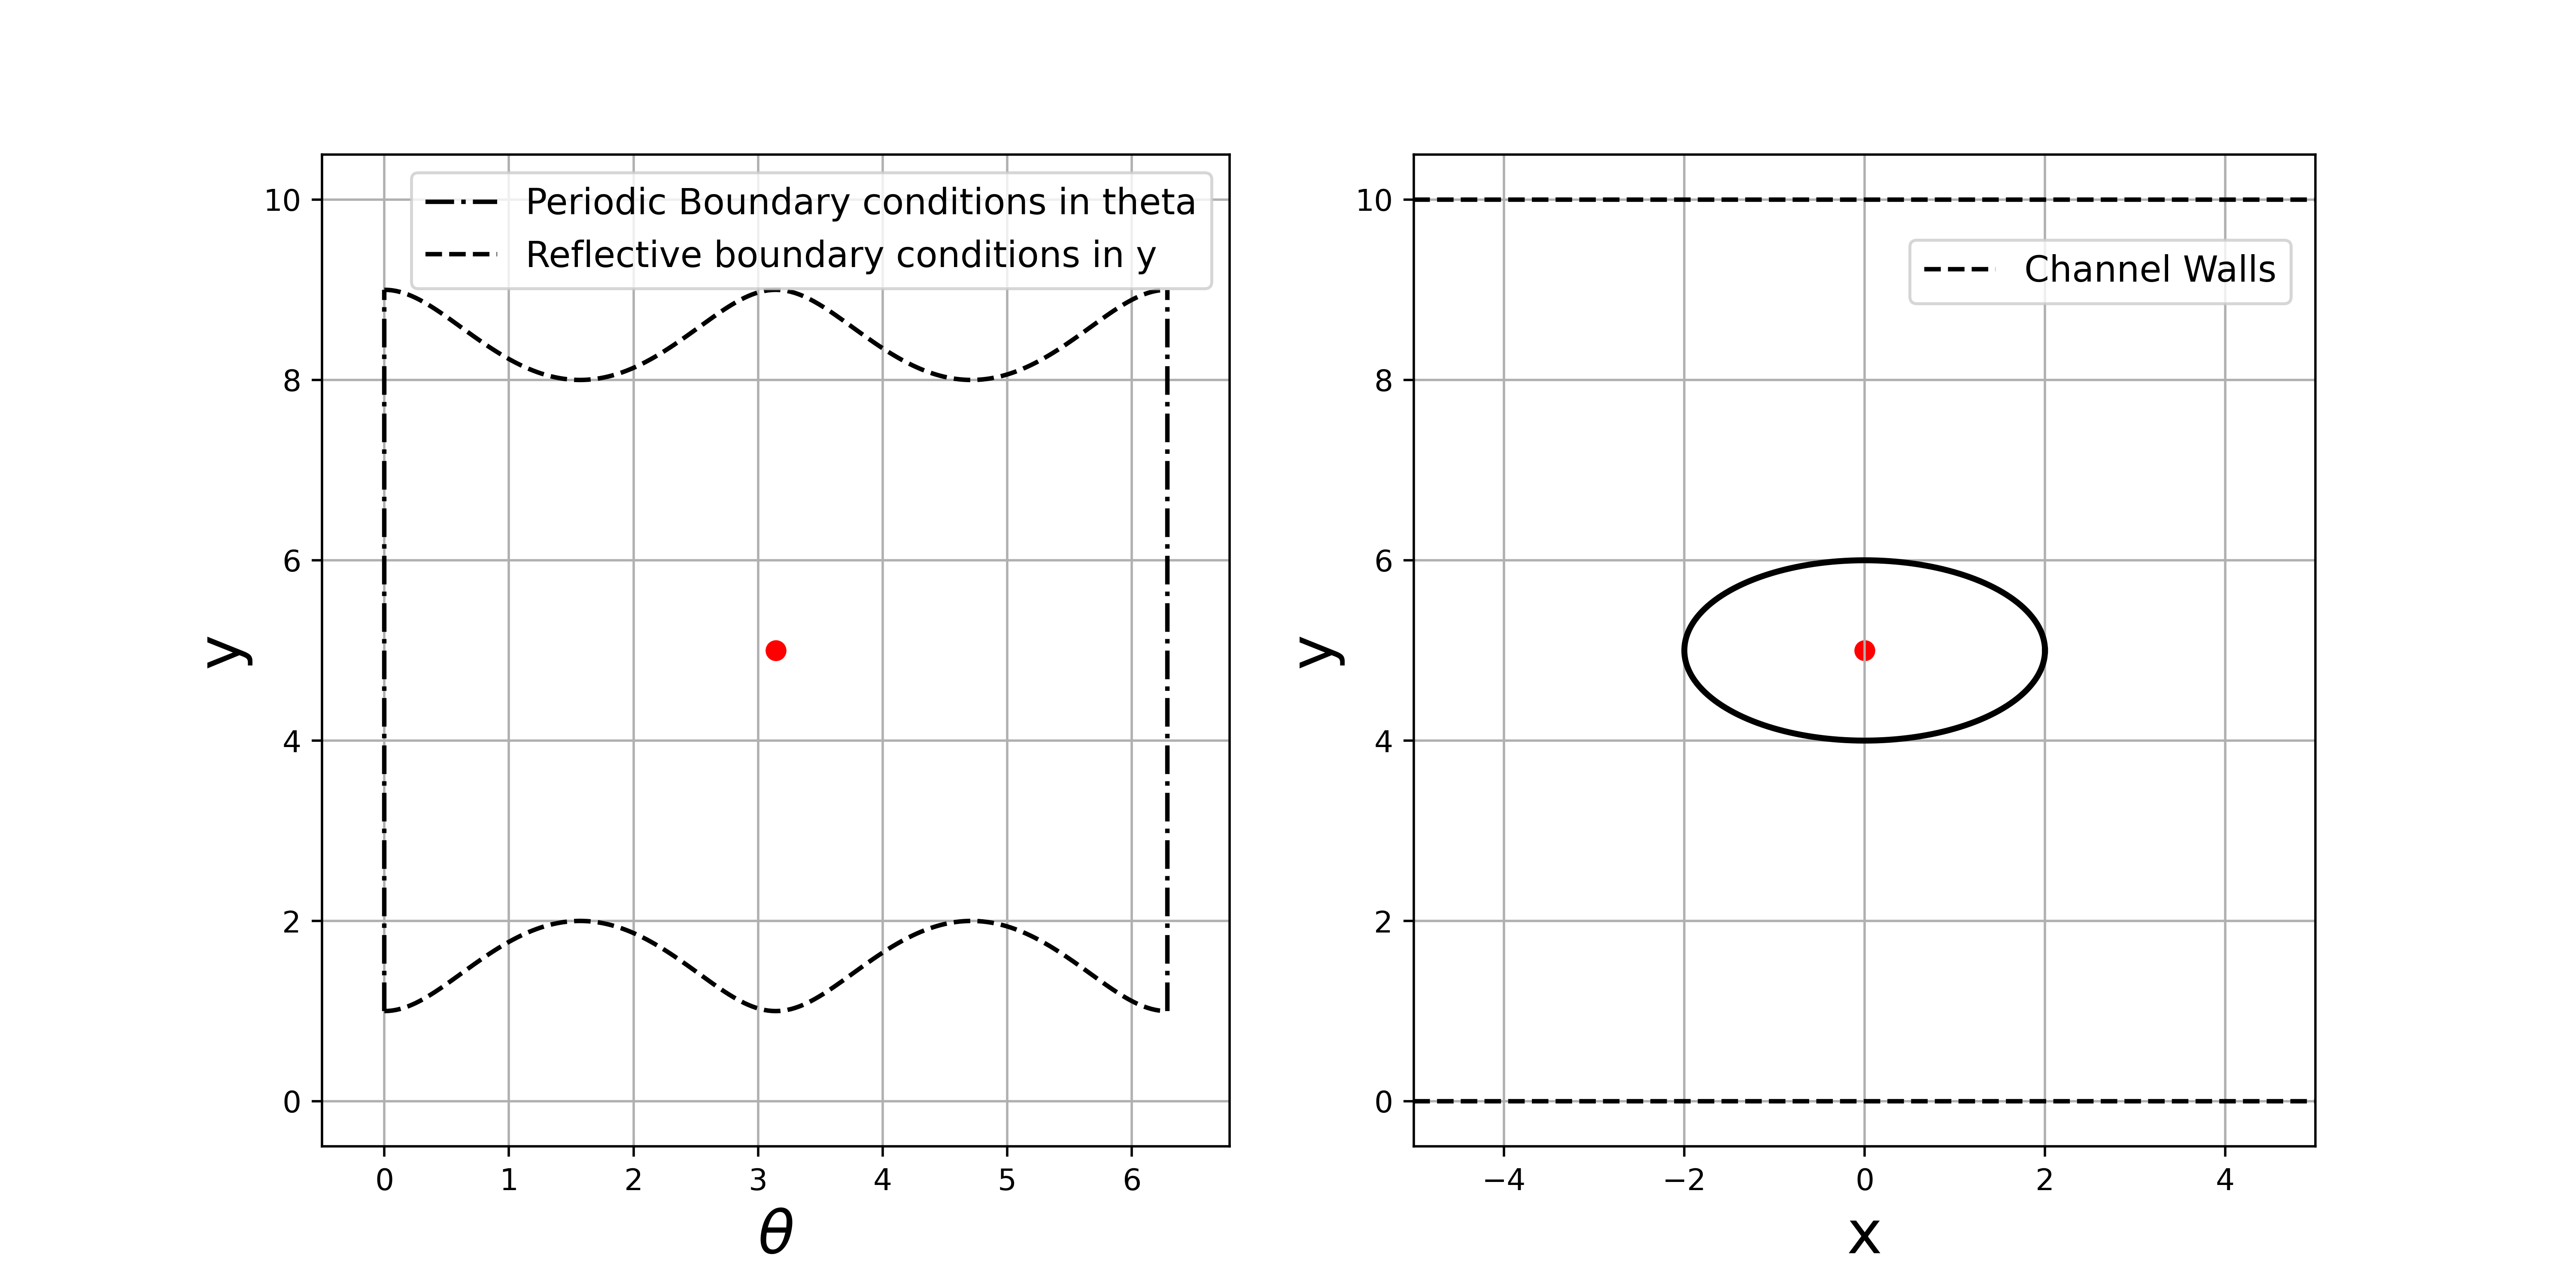
\includegraphics[scale=0.45]{graphics/config_space_1.png}
    \caption{Configuration space for Model 1 and its correspondance to 
    the physical system of a cell within a channel. Parameters used: $a=2$, $b=1$, $H=10$}
    \label{fig:configuration_space_model_1}
\end{figure}

Figure \ref{fig:configuration_space_model_1} also shows the boundary conditions 
applied to the configuration space. Periodic boundary conditions on the orientation variable
$\theta$ at $\theta=0$ and $\theta=2\pi$, while reflective boundary conditions are applied
at the upper and lower boundaries described by $y_{min}(x)$ and $y_{max}(x)$.

With a clearly bounded configuration space, the corresponding 
Fokker-Planck equation associated with equations \eqref{eq:model1_sdes} can be solved. The corresponding Fokker-Planck
equation is:

\begin{equation}\label{eq:model_1_fokker_planck}
    \frac{\partial p}{\partial t} = -\frac{\partial}{\partial y} (U\sin(\theta) p) 
    + D_{\theta} \frac{\partial^2 p}{\partial \theta^2} 
    + D_y \frac{\partial^2 p}{\partial y^2}
\end{equation}


When solving equation \eqref{eq:model_1_fokker_planck}, no-flux boundary conditions are applied at the upper and lower
boundaries along the $y$-axis, accounting for the conservation of probability within the domain. 
The finite element solver COMSOL Multiphysics\textregistered was used to numerically obtain the stationary distribution 
\cite{comsol}. The resulting PDF is presented in Figure \ref{fig:subfig_model_1_pdf}, and the resulting marginal 
distribution across the channel is displayed in Figure \ref{fig:subfig_model_1_marginal_y}.


\begin{figure}[htbp]
    \centering
    \begin{subfigure}[b]{0.45\textwidth}
        \centering
        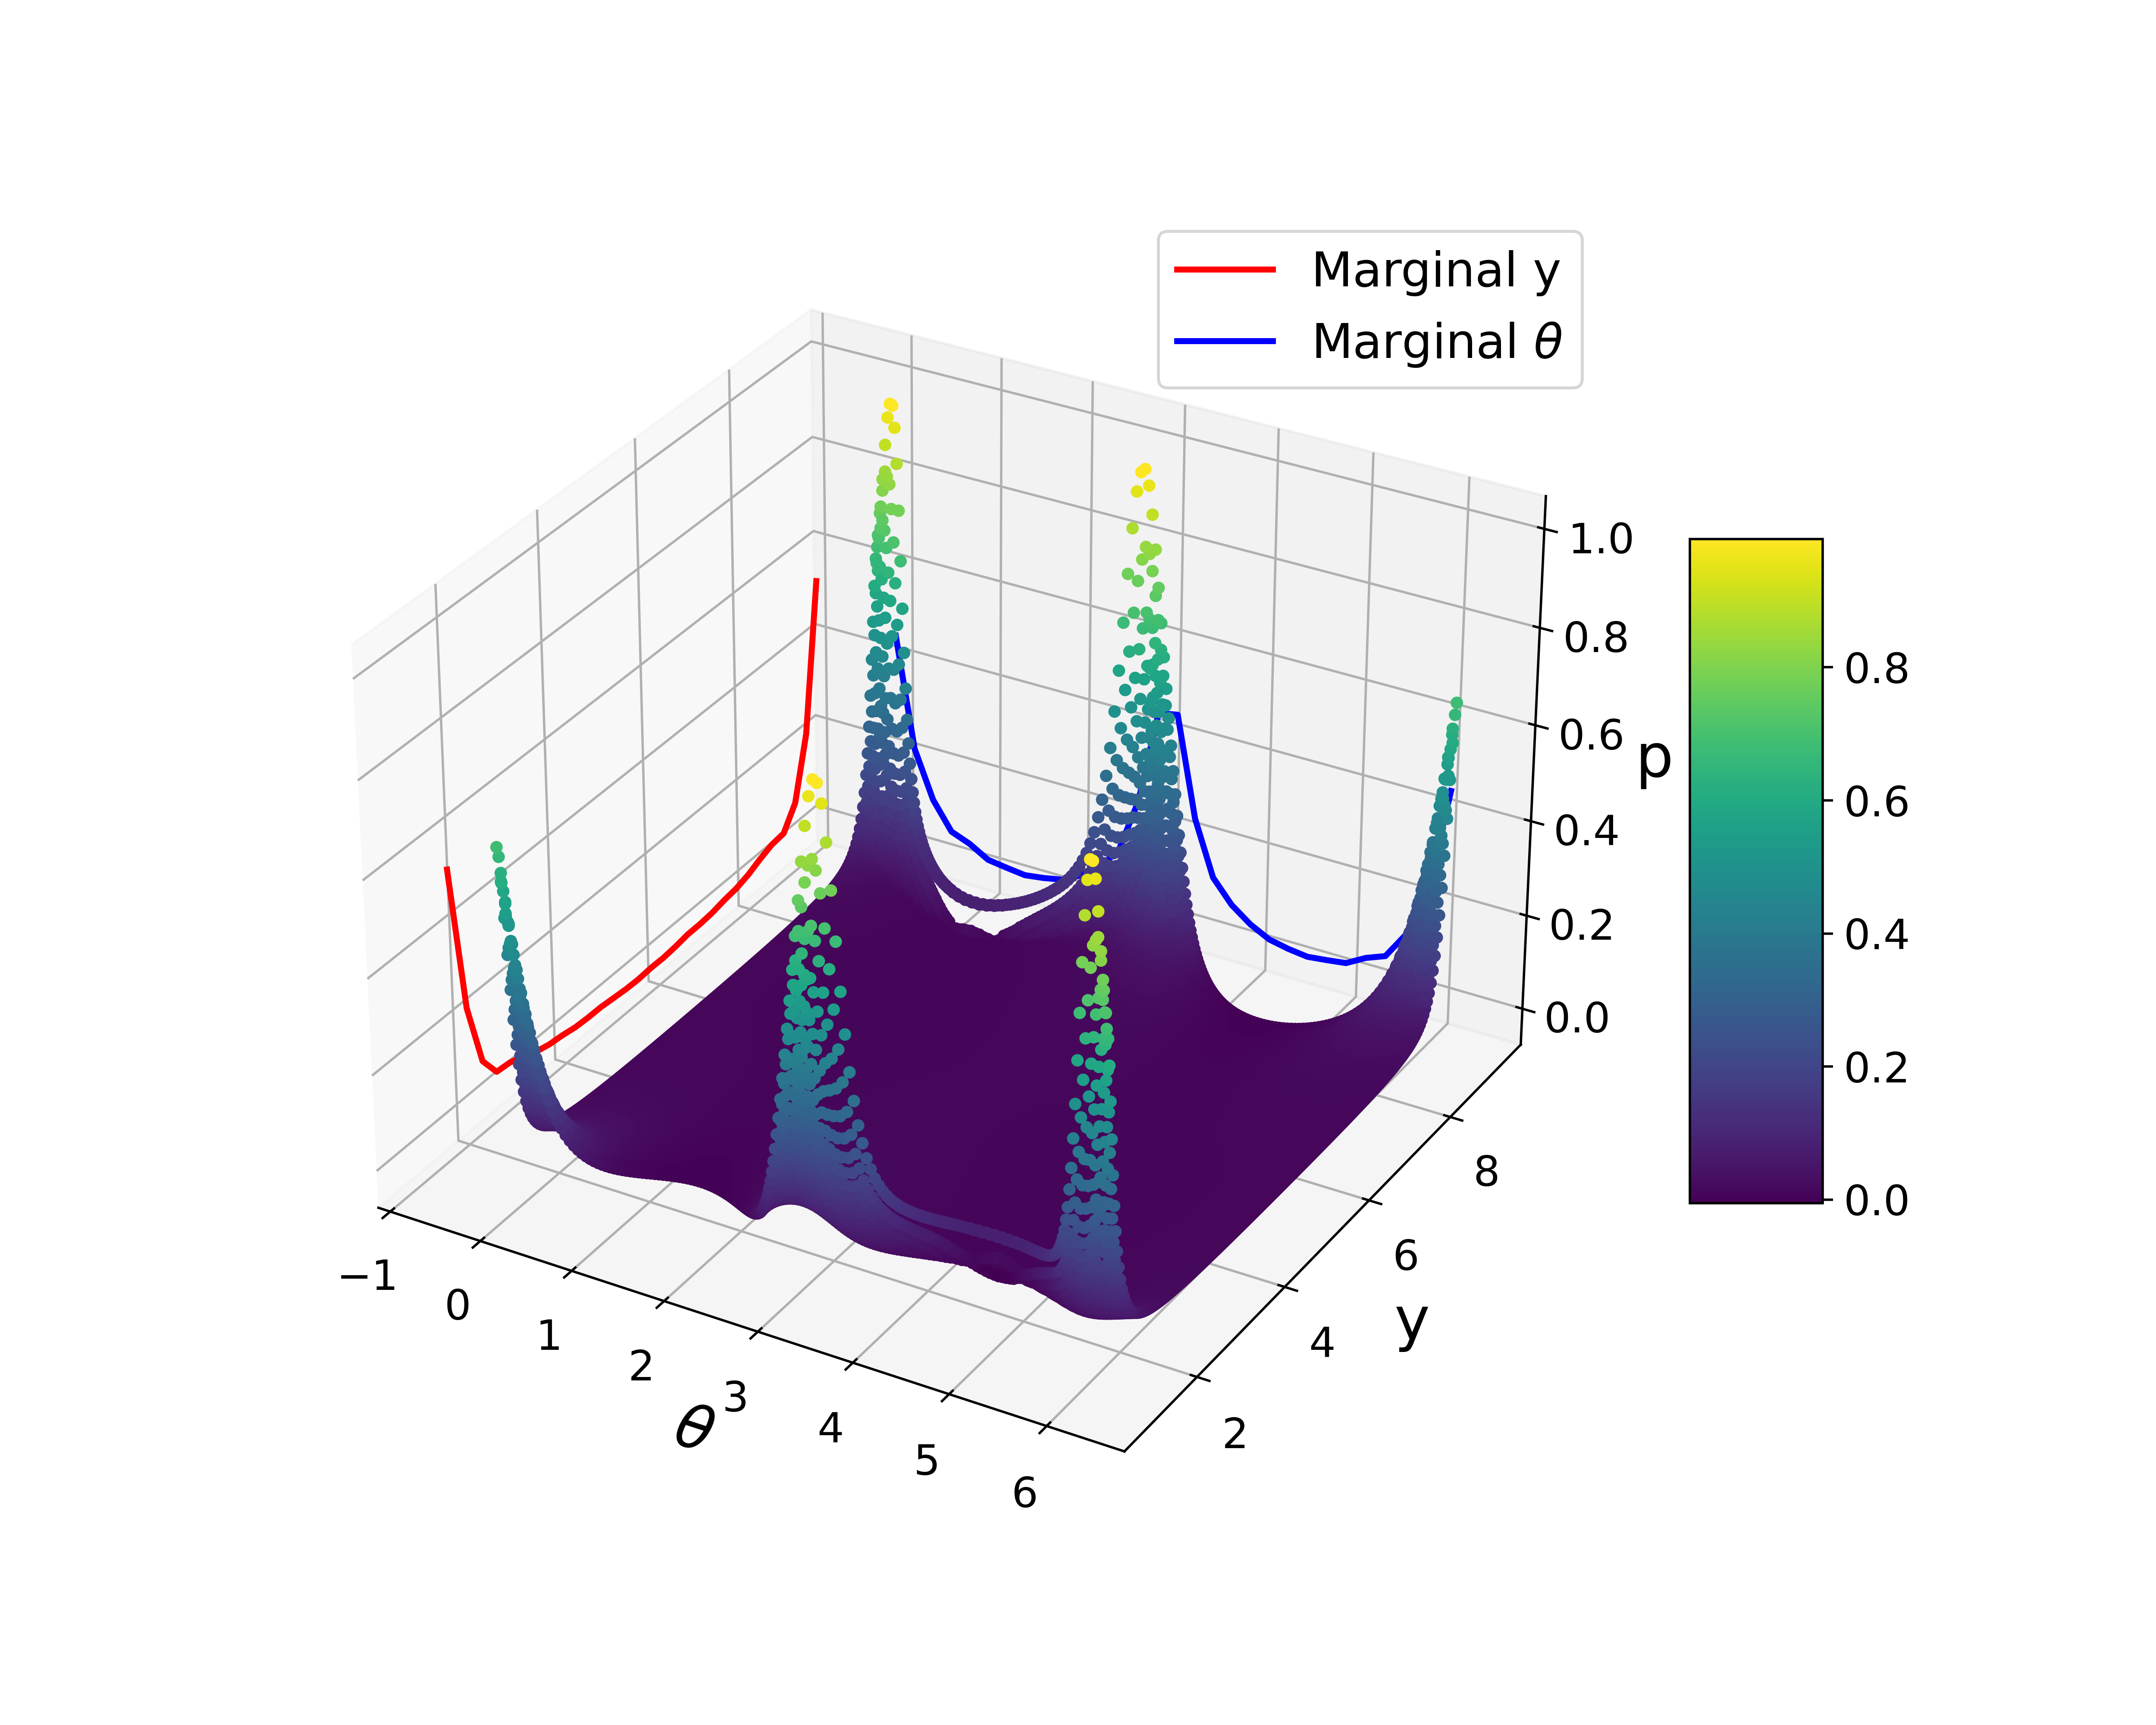
\includegraphics[width=\textwidth, trim=30 20 30 20, clip]{graphics/model_1_pdf_surface.png}
        \caption{Stationary distribution obtained for equations \eqref{eq:model1_sdes}. Marginal distributions are displayed along 
        the axes margins.}
        \label{fig:subfig_model_1_pdf}
    \end{subfigure}
    \hfill
    \begin{subfigure}[b]{0.45\textwidth}
        \centering
        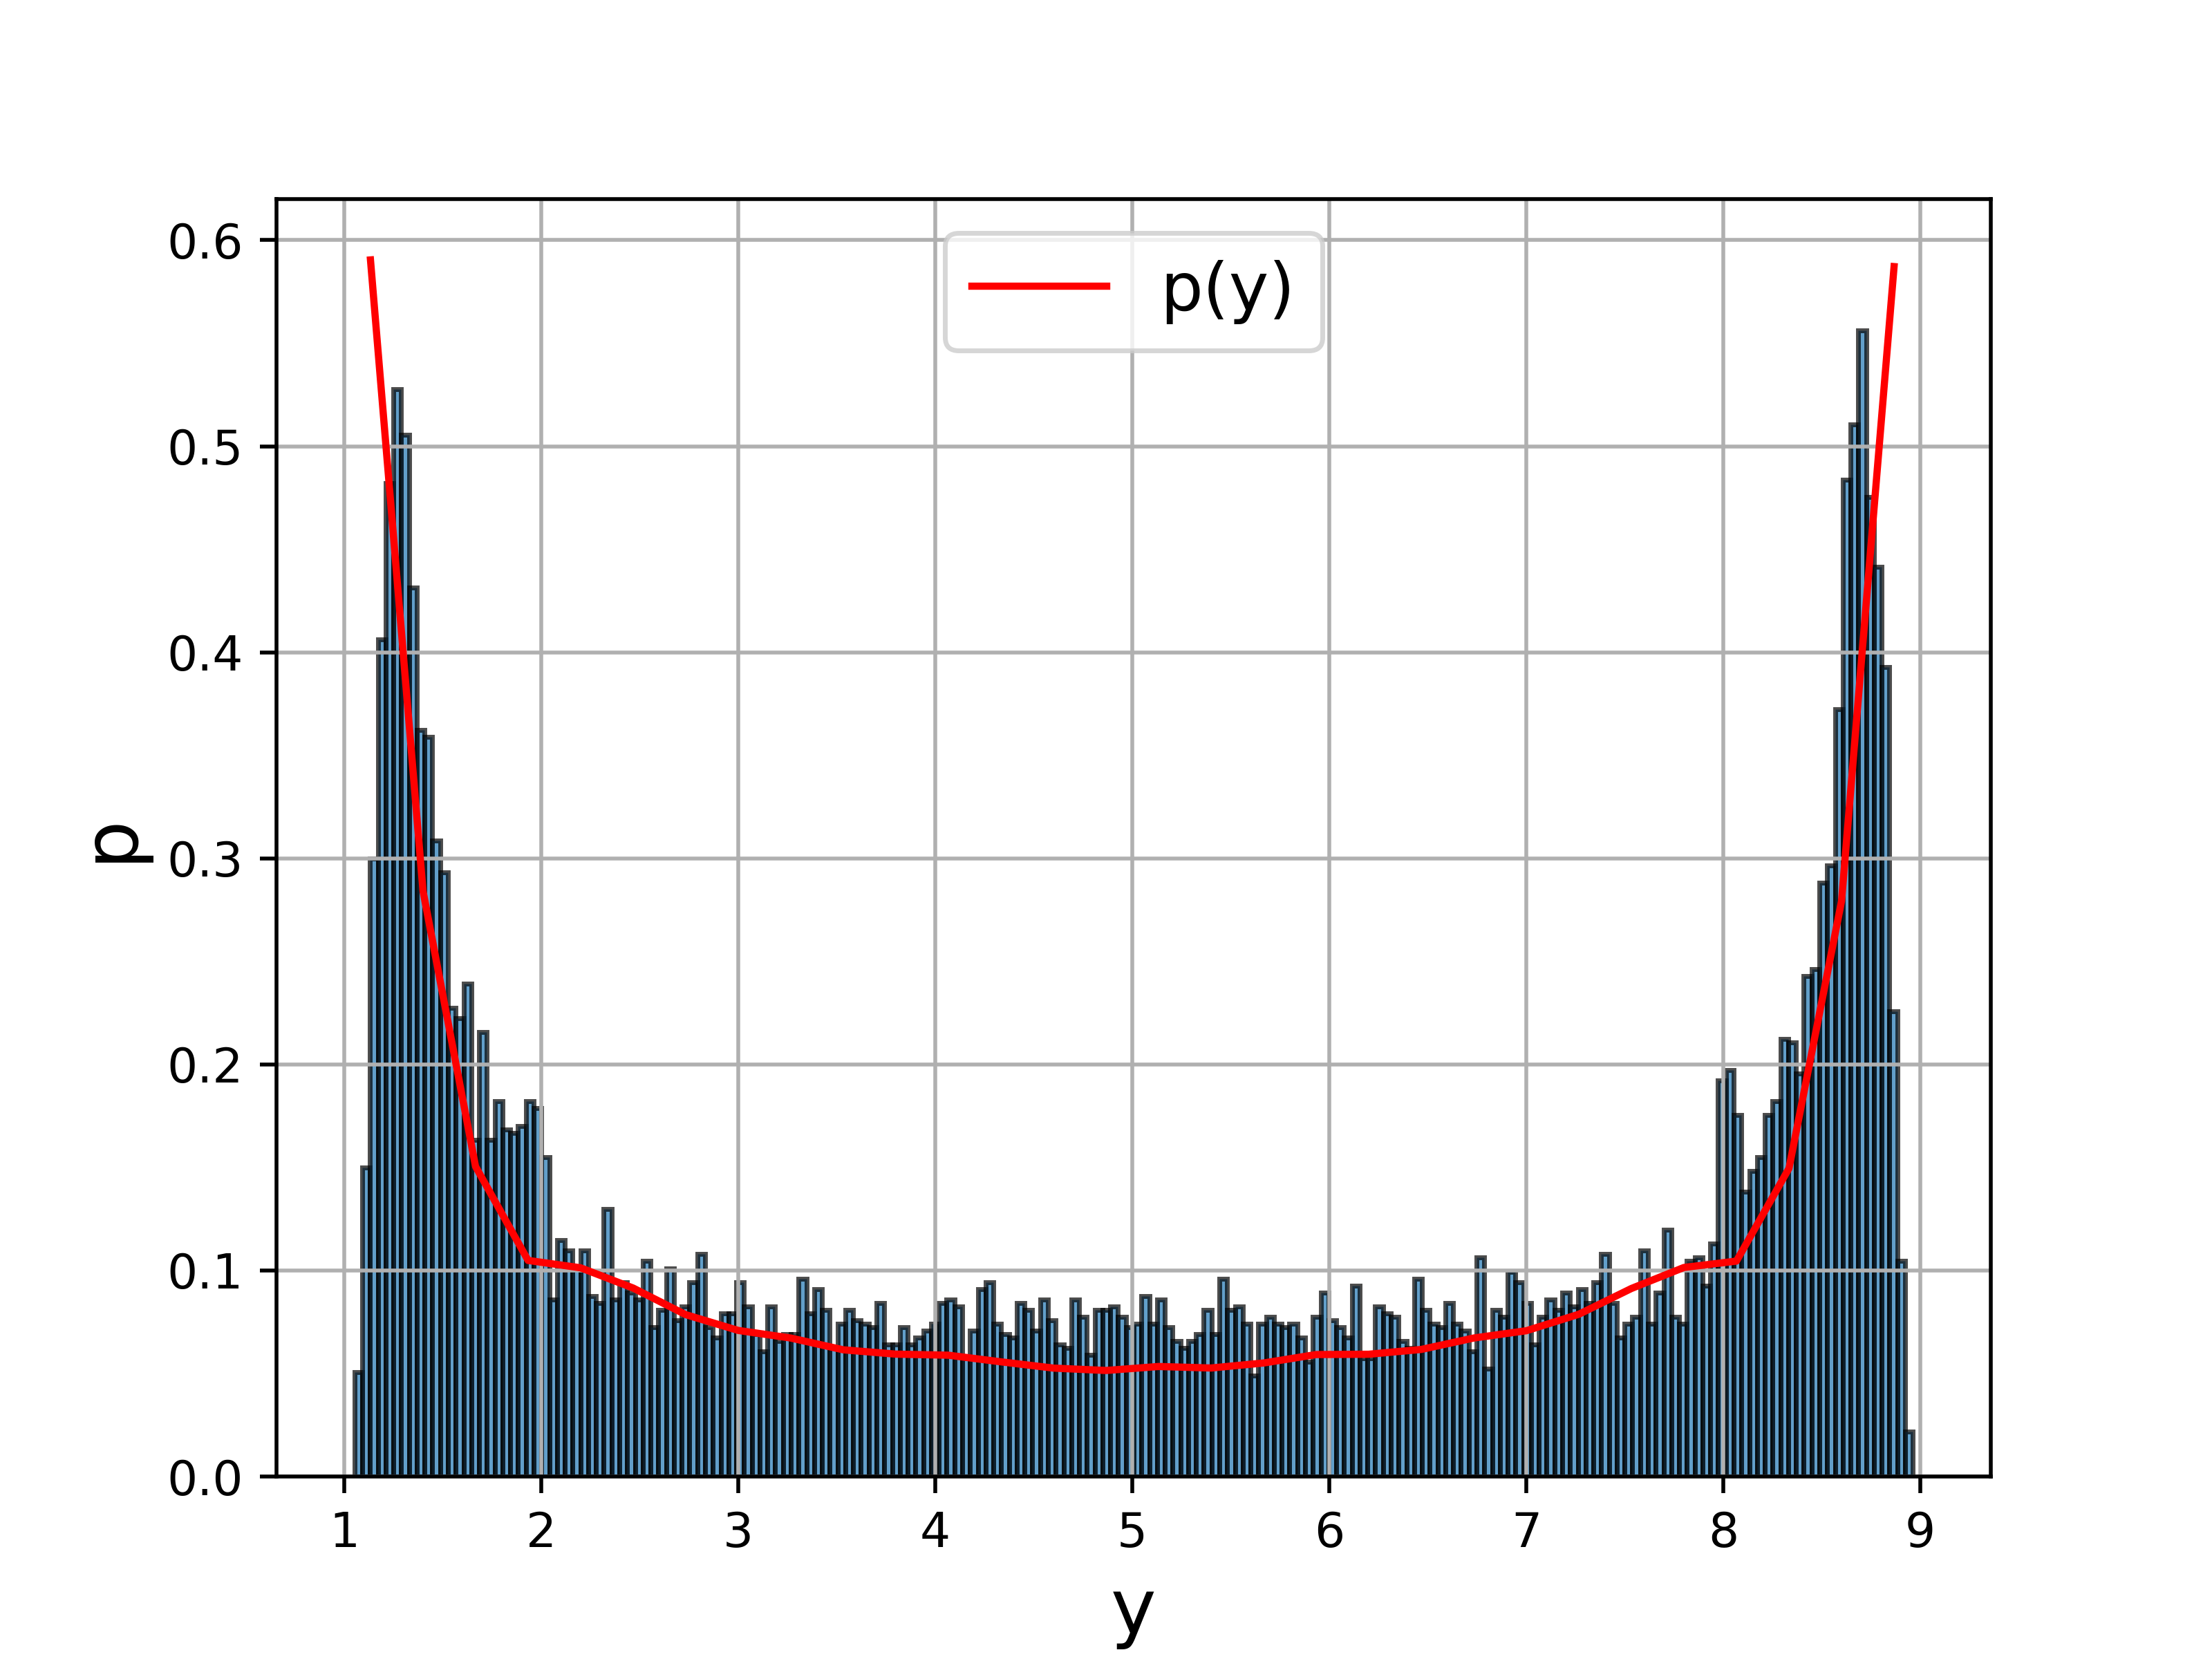
\includegraphics[width=\textwidth]{graphics/model_1_marginal_y.png}
        \caption{Marginal distributions along $y$ derived from solving the Fokker-Planck (red line) and from
         Monte Carlo simulation (histogram)}
        \label{fig:subfig_model_1_marginal_y}
    \end{subfigure}
    \caption{Comparison of stationary distribution and its marginal along $y$.}
    \label{fig:model_1_results}
\end{figure}

The marginal distribution along the $y$-axis clearly exhibits characteristic boundary accumulation behaviour. 
We attribute this phenomenon as arising from two primary mechanisms. Firstly, the drift term in equation \eqref{eq:model1_sdes_a} 
implies that, on average, the cell moves towards and eventually encounters the boundary, where it becomes constrained 
until it sufficiciently reorients. Secondly, the geometry of the configuration space contributes significantly; the elliptical
shape introduces two "hills" with reflective boundaries. These features act as barriers, hindering the ease with 
which the system can exit the boundary regions, thus enhacing the boundary accummulation.